\phantomsection\numberedsection{RF5.1 Crear relación}

\subsection*{Descripción}
Permite a los usuarios definir nuevas relaciones para poder relacionar productos con otros y sugerirlos de una forma más rápida.\par
\vspace{0.15cm}

\textbf{Pre-condición}\par
El usuario ha iniciado sesión en su cuenta en Mini PIM y no tiene la máxima capacidad de relaciones creadas establecidas su plan de suscripción\footnote{Todos los casos de uso están pensados para seguir el plan gratuito. El total de relaciones permitidas en este plan son 3.}.\par
\vspace{0.15cm}

\textbf{Post-condición}
\begin{itemize}
    \item Caso de éxito: La relación es creada correctamente, se muestra en la lista de relaciones con el nombre ingresado.
    \item Caso mínimo: El sistema notifica al usuario el resultado de la acción de crear relación: exitosa o fallida.
\end{itemize}

\textbf{Prioridad: }
Alta
\vspace{0.15cm}

\textbf{Autores: }
Pablo Ortega Serapio y Francisco Javier Jordá Garay\par
\vspace{0.15cm}

\textbf{Control de cambios: } Versión 1: Definición del caso de uso

\numberedsubsection{Escenario principal}
\begin{enumerate}
    \item El usuario ha iniciado sesión con su cuenta de usuario correspondiente.
    \item El usuario accede a la sección de \enquote{Relaciones}.
    \item El sistema muestra la lista de relaciones existentes y la opción para crear una nueva.
    \item El usuario selecciona la opción \enquote{Añadir relación} crear una nueva relación.
    \item El sistema muestra el menú de creación de relación.
    \item El usuario ingresa el nombre deseado y selecciona los productos que quiere que se relacionen.
    \item El sistema verifica que el nombre de la relación no sea erróneo\footnote{Se considera erróneo cualquier nombre que este vacío, no sea único o sea igual a algún GTIN o algún SKU del sistema.}.
    \item El sistema verifica que si se selecciona un producto de la columna izquierda, también debe haber un producto seleccionado en la columna derecha para poder crear la relación\footnote{No permitimos en nuestro sistema relacionar un producto a \emph{null}. O la relación está vacía (sin productos seleccionas) o si se selecciona un producto, debe tener como mínimo alguno relacionado.}.
    \item El sistema crea la nueva relación y actualiza la lista de relaciones para incluirla.
    \item El sistema muestra la lista de relaciones con la nueva relación añadida.
\end{enumerate}

\numberedsubsection{Escenarios alternativos}
\begin{description}

    \item[4.a] El sistema no permite crear relaciones.
    \begin{enumerate}
        \item[4.a.1] El sistema no permite crear relaciones adicionales inhabilitando el botón de \enquote{Añadir relación} hasta que se eliminen relaciones existentes.
        \item[4.a.2] El sistema muestra un mensaje indicando que no se pueden crear nuevas relaciones. 
    \end{enumerate}
    
    \item[7.a] El sistema detecta que el nombre de la relación es erróneo.
    \begin{enumerate}
        \item[7.a.1] El sistema muestra un mensaje de error indicando que el nombre no es válido.
        \item[7.a.2] El sistema devuelve al usuario al menú de creación de relación permitiendo modificar el nombre.
    \end{enumerate}
    
    \item[8.a] El sistema detecta que solo hay elementos seleccionados en la columna izquierda.
    \begin{enumerate}
        \item[8.a.1] El sistema muestra un mensaje de error solicitando que seleccione un producto de la tabla derecha o que se deseleccionen los productos de la columna izquierda.
        \item[8.a.2] El sistema devuelve al usuario al menú de creación de relación para continuar eligiendo productos.
    \end{enumerate}

    \item[*.a] El usuario cancela la acción de crear una relación nueva cerrando el menú de creación de relación.
    \begin{enumerate}
        \item[*.a.1] El sistema regresa a la sección de \enquote{Relaciones}.
    \end{enumerate}
\end{description}

\numberedsubsection{Casos de Prueba}
\underline{Escenario: Principal}\par
\vspace{0.15cm}
\textbf{Dado} que el usuario ha iniciado sesión con su cuenta de usuario correspondiente,\par
\textbf{Y} no ha alcanzado el número máximo de relaciones creadas,\par
\textbf{Y} está en el apartado de \enquote{Relaciones},\par
\textbf{Cuando} selecciona la opción \enquote{Añadir relación},\par
\textbf{E} ingresa correctamente el nombre de la relación que desea crear,\par
\textbf{Y} selecciona correctamente los productos en las columnas de izquierda y derecha,\par
\textbf{Y} selecciona \enquote{Confirmar} para guardar los datos,\par
\textbf{Entonces} el sistema almacena la información de la nueva relación,\par
\textbf{Y} actualiza la lista de relaciones para incluir la nueva relación creada,\par
\textbf{Y} muestra el apartado de \enquote{Relaciones} con todas las relaciones.\par

\vspace{0.20cm}

\underline{Escenario: Alternativo 4.a (límite de relaciones alcanzado)}\par
\vspace{0.15cm}
\textbf{Dado} que el usuario ha iniciado sesión con su cuenta de usuario correspondiente,\par
\textbf{Y} ha alcanzado el número máximo de relaciones creadas,\par
\textbf{Y} está en el apartado de \enquote{Relaciones},\par
\textbf{Cuando} el usuario intenta crear una nueva relación,\par
\textbf{Entonces} el sistema no le inhabilita el botón de \enquote{Añadir relación},\par
\textbf{Y} muestra un mensaje indicando que no se pueden crear nuevas relaciones,\par
\textbf{Y} no le permite crear más relaciones hasta que se eliminen relaciones existentes.\par

\vspace{0.20cm}
\newpage % Para que el caso alternativo 7 se vea completo en una página

\underline{Escenario: Alternativo 7.a (nombre de relación erróneo)}\par
\vspace{0.15cm}
\textbf{Dado} que el usuario ha iniciado sesión con su cuenta de usuario correspondiente,\par
\textbf{Y} no ha alcanzado el número máximo de relaciones creadas,\par
\textbf{Y} está en el apartado de \enquote{Relaciones},\par
\textbf{Cuando} el usuario selecciona la opción \enquote{Añadir relación},\par
\textbf{E} ingresa un nombre erróneo para la relación,\par
\textbf{Entonces} el sistema notifica al usuario que el nombre de la relación es erróneo,\par
\textbf{Y} muestra un mensaje de error indicando que el nombre no es válido,\par
\textbf{Y} devuelve al usuario al menú de creación de relación permitiendo modificar el nombre.\par

\vspace{0.20cm}

\underline{Escenario: Alternativo 8.a (productos no seleccionados correctamente)}\par
\vspace{0.15cm}
\textbf{Dado} que el usuario ha iniciado sesión con su cuenta de usuario correspondiente,\par
\textbf{Y} no ha alcanzado el número máximo de relaciones creadas,\par
\textbf{Y} está en el apartado de \enquote{Relaciones},\par
\textbf{Cuando} el usuario selecciona la opción \enquote{Añadir relación},\par
\textbf{Y} selecciona productos de forma errónea,\par
\textbf{Entonces} el sistema muestra un mensaje de error indicando que debe seleccionar productos correctamente en ambas columnas,\par
\textbf{Y} devuelve al usuario al menú de creación de relación para continuar seleccionando productos.\par

\vspace{0.20cm}


\underline{Escenario: Alternativo *.a (cancelación de la creación de una nueva relación)}\par
\vspace{0.15cm}
\textbf{Dado} que el usuario ha iniciado sesión con su cuenta de usuario correspondiente,\par
\textbf{Y} no ha alcanzado el número máximo de relaciones creadas,\par
\textbf{Y} está en el apartado de \enquote{Relaciones},\par
\textbf{Cuando} el usuario selecciona la opción \enquote{Añadir relación},\par
\textbf{Y} el usuario decide cancelar la creación de la relación seleccionando la opción de cerrar el menú de creación,\par
\textbf{Entonces} el sistema regresa al apartado de \enquote{Relaciones},\par
\textbf{Y} muestra el listado de relaciones existentes sin ningún cambio realizado.\par

\vspace{0.20cm}

\numberedsubsection{Bocetos}
\begin{figure}[H]
    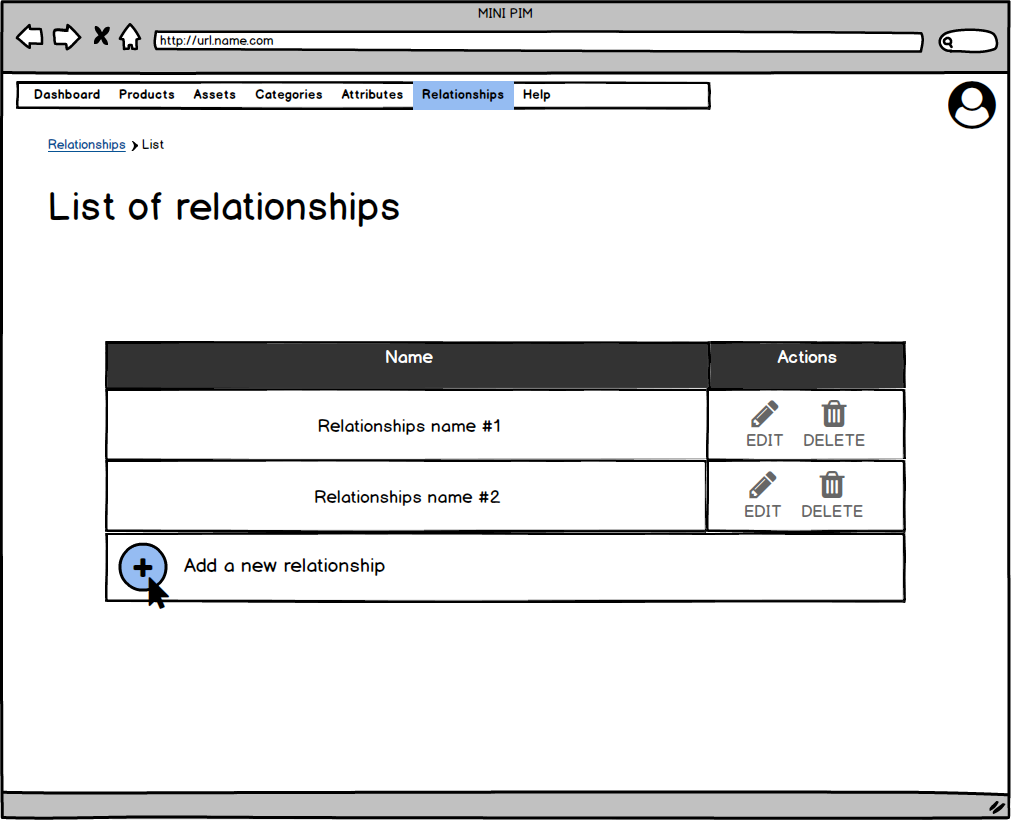
\includegraphics[width=1\linewidth]{assets/mockups/RF5.1_1.png}
    \caption{Sección de \enquote{Relaciones}}
   \end{figure}
\vspace{1.0cm}

\begin{figure}[H]
    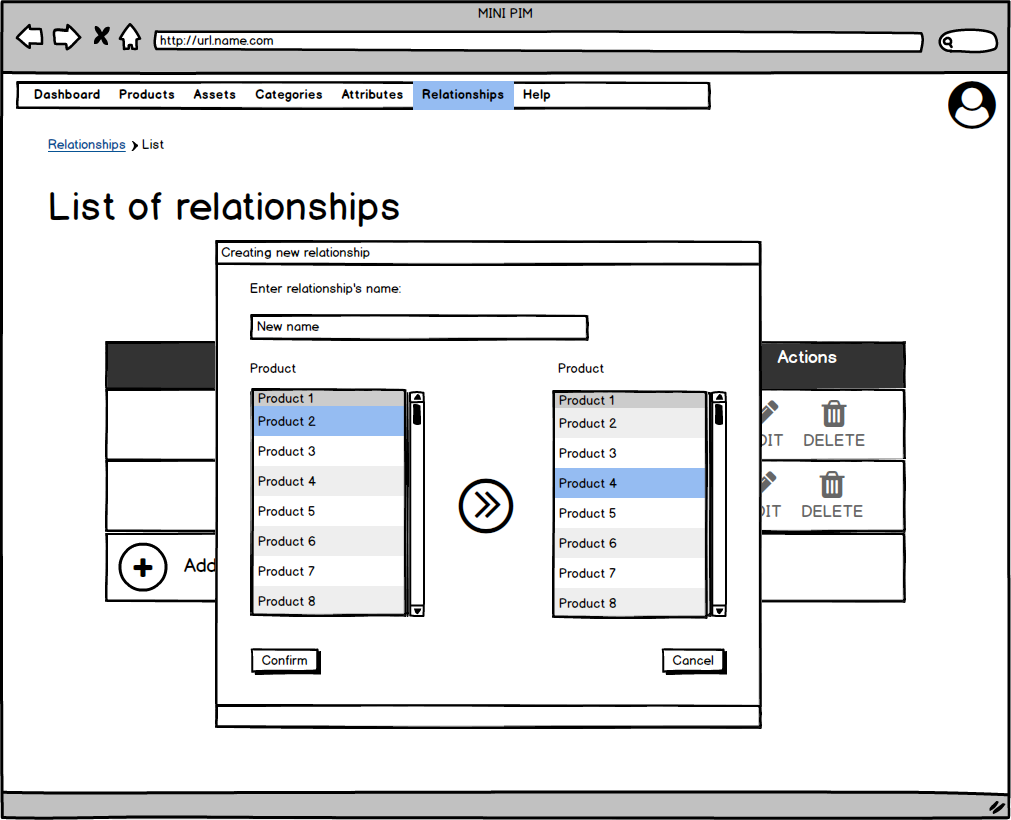
\includegraphics[width=1\linewidth]{assets/mockups/RF5.1_2.png}
    \caption{Menú de creación de relación tras clicar la opción \enquote{Añadir relación}}
   \end{figure}
\vspace{1.0cm}

\begin{figure}[H]
    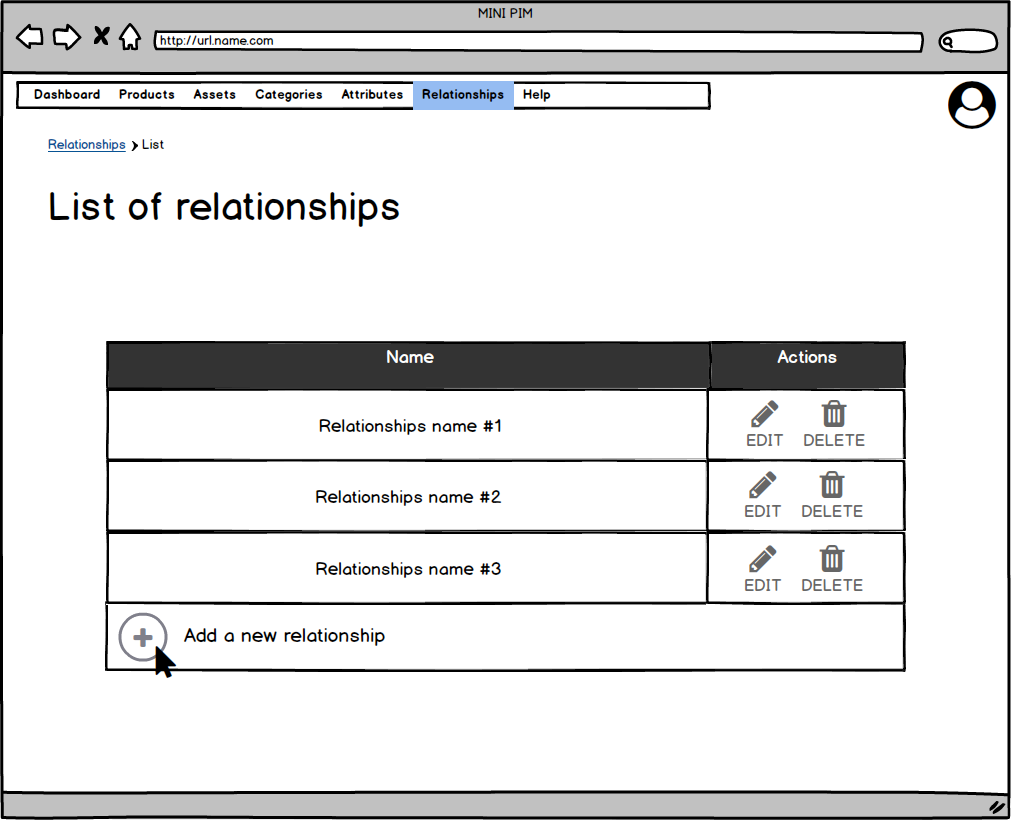
\includegraphics[width=1\linewidth]{assets/mockups/RF5.1_3.png}
    \caption{Escenario con al máximo de relaciones creadas}
   \end{figure}
\vspace{1.0cm}

\newpage % Muestra el diagrama de secuencias en una nueva página

\numberedsubsection{Diagrama de Secuencia (por hacer)}
\begin{figure}[H]
    
\includegraphics[width=1\linewidth]{assets/umaLogo.png}
    \caption{Escenario principal para crear el Informe de Cuenta}
   \end{figure}
\vspace{1.0cm}

\newpage % Inicia en una nueva página otro caso de uso